%% Creator: Inkscape 1.0.2 (e86c8708, 2021-01-15), www.inkscape.org
%% PDF/EPS/PS + LaTeX output extension by Johan Engelen, 2010
%% Accompanies image file 'res/skin-H-Weg.pdf' (pdf, eps, ps)
%%
%% To include the image in your LaTeX document, write
%%   \input{<filename>.pdf_tex}
%%  instead of
%%   \includegraphics{<filename>.pdf}
%% To scale the image, write
%%   \def\svgwidth{<desired width>}
%%   \input{<filename>.pdf_tex}
%%  instead of
%%   \includegraphics[width=<desired width>]{<filename>.pdf}
%%
%% Images with a different path to the parent latex file can
%% be accessed with the `import' package (which may need to be
%% installed) using
%%   \usepackage{import}
%% in the preamble, and then including the image with
%%   \import{<path to file>}{<filename>.pdf_tex}
%% Alternatively, one can specify
%%   \graphicspath{{<path to file>/}}
%% 
%% For more information, please see info/svg-inkscape on CTAN:
%%   http://tug.ctan.org/tex-archive/info/svg-inkscape
%%
\begingroup%
\makeatletter%
\def\svgwidth{0.5\textwidth}
\providecommand\color[2][]{%
	\errmessage{(Inkscape) Color is used for the text in Inkscape, but the package 'color.sty' is not loaded}%
	\renewcommand\color[2][]{}%
}%
\providecommand\transparent[1]{%
	\errmessage{(Inkscape) Transparency is used (non-zero) for the text in Inkscape, but the package 'transparent.sty' is not loaded}%
	\renewcommand\transparent[1]{}%
}%
\providecommand\rotatebox[2]{#2}%
\newcommand*\fsize{\dimexpr\f@size pt\relax}%
\newcommand*\lineheight[1]{\fontsize{\fsize}{#1\fsize}\selectfont}%
\ifx\svgwidth\undefined%
	\setlength{\unitlength}{841.88976378bp}%
	\ifx\svgscale\undefined%
		\relax%
	\else%
		\setlength{\unitlength}{\unitlength * \real{\svgscale}}%
	\fi%
\else%
	\setlength{\unitlength}{\svgwidth}%
\fi%
\global\let\svgwidth\undefined%
\global\let\svgscale\undefined%
\makeatother%
\begin{picture}(1,0.70707071)%
	\tiny
	\lineheight{1}%
	\setlength\tabcolsep{0pt}%
	\put(0,0){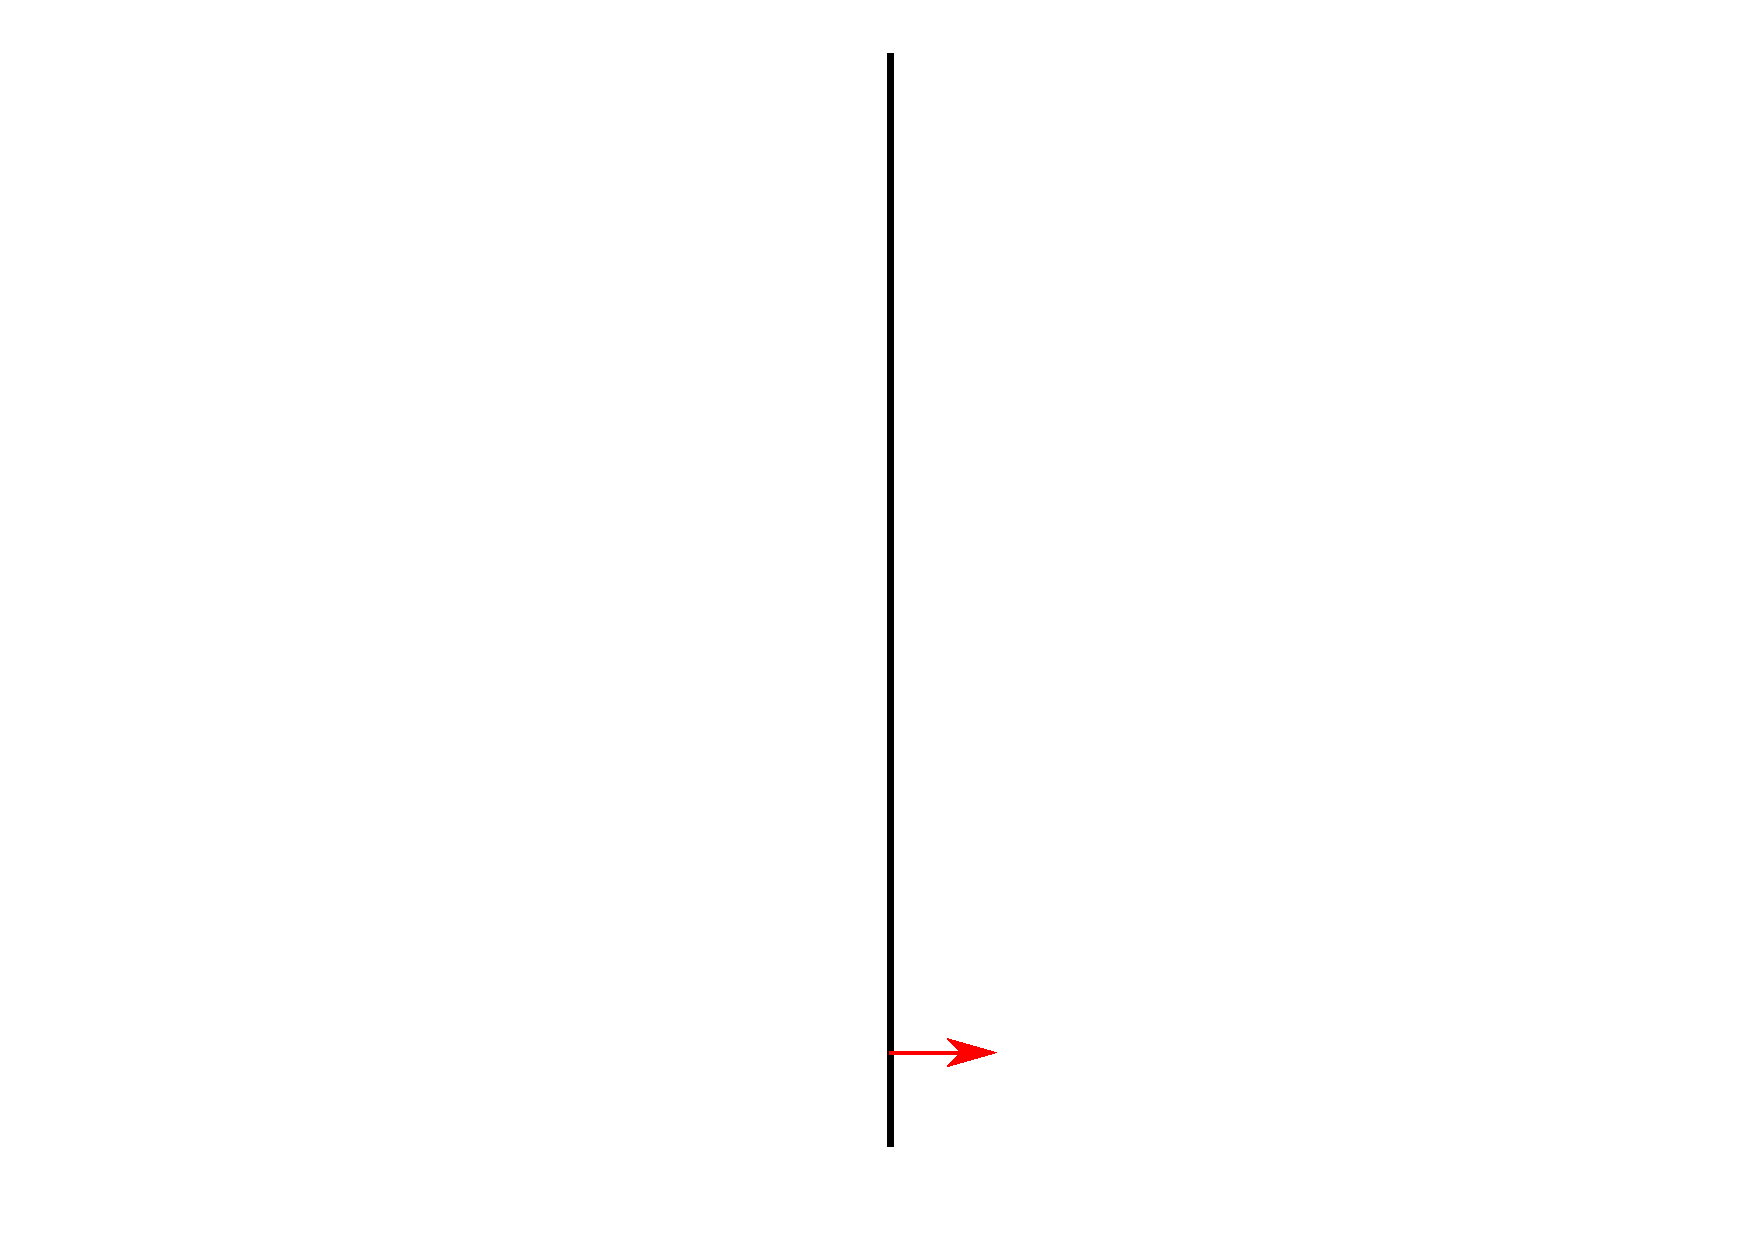
\includegraphics[width=\unitlength,page=1]{res/skin-H-Weg.pdf}}%
	\put(0.58209141,0.09491588){\color[rgb]{0.98823529,0,0}\makebox(0,0)[lt]{\lineheight{1.25}\smash{\begin{tabular}[t]{l}x\end{tabular}}}}%
	\put(0,0){\includegraphics[width=\unitlength,page=2]{res/skin-H-Weg.pdf}}%
	\put(0.46827199,0.1318683){\color[rgb]{0.98823529,0,0}\makebox(0,0)[lt]{\lineheight{1.25}\smash{\begin{tabular}[t]{l}y\end{tabular}}}}%
	\put(0.46795675,0.04442039){\color[rgb]{0.98823529,0,0}\makebox(0,0)[lt]{\lineheight{1.25}\smash{\begin{tabular}[t]{l}z\end{tabular}}}}%
	\put(0,0){\includegraphics[width=\unitlength,page=3]{res/skin-H-Weg.pdf}}%
	\put(0.3165163,0.59414568){\color[rgb]{0,0,0}\makebox(0,0)[lt]{\lineheight{1.25}\smash{\begin{tabular}[t]{l}$\kappa = 0$\end{tabular}}}}%
	\put(0.53121635,0.59414568){\color[rgb]{0,0,0}\makebox(0,0)[lt]{\lineheight{1.25}\smash{\begin{tabular}[t]{l}$\kappa \ne 0$\end{tabular}}}}%
	\put(0,0){\includegraphics[width=\unitlength,page=4]{res/skin-H-Weg.pdf}}%
	\put(0.19130244,0.39197271){\color[rgb]{0,0,0}\makebox(0,0)[lt]{\lineheight{1.25}\smash{\begin{tabular}[t]{l}$\vec{J} = \vec{0}$\end{tabular}}}}%
	\put(0.57126733,0.3923207){\color[rgb]{0,0,0}\makebox(0,0)[lt]{\lineheight{1.25}\smash{\begin{tabular}[t]{l}$\vec{J} = J_y(x) \vu{y}$\end{tabular}}}}%
	\put(0.85455836,0.20060427){\color[rgb]{0,0,0}\makebox(0,0)[lt]{\lineheight{1.25}\smash{\begin{tabular}[t]{l}$x \to \infty$\end{tabular}}}}%
	\put(0.02758345,0.39143333){\color[rgb]{0,0,0}\makebox(0,0)[lt]{\lineheight{1.25}\smash{\begin{tabular}[t]{l}$\zeta$\end{tabular}}}}%
\end{picture}%
\endgroup%
